\documentclass[aspectratio=169]{ctexbeamer}
\definecolor{urls}{RGB}{137, 180, 250}
\definecolor{link_text}{RGB}{245, 224, 220}
\hypersetup{
  colorlinks,
  linkcolor=link_text,
  urlcolor=urls,
}
\renewcommand{\UrlFont}{\ttfamily\scriptsize}

\usetheme{AnnArbor}
\usepackage[style=Mocha,accent=Rosewater]{beamercolorthemecatppuccin}

\usefonttheme{serif}
\usefonttheme{professionalfonts}

\usepackage[T1]{fontenc}
\setmainfont{LXGW WenKai}
% \setmainfont{Cascadia Code NF}
% \setsansfont{}
\setmonofont{Cascadia Code NF}
\usepackage{xeCJK}
\setCJKmainfont{LXGW WenKai}
% \setCJKmainfont{}
\setCJKmonofont{Cascadia Code NF}
\newcommand{\nerd}[1]{\texttt{#1}}
\setmonofont{Cascadia Code NF}[
  Contextuals=Alternate
]

\PassOptionsToPackage{hyphens}{url}
% \usepackage{ulem}
\usepackage{graphicx}
%\usepackage{wrapfig}
\usepackage{pifont} % Symbols used as itemize symbols
\usepackage{enumitem}
\setlist[itemize,1]{label={\small\color[RGB]{242, 205, 205}\ding{111}}}
\setlist[itemize,2]{label={\footnotesize\color[RGB]{242, 205, 205}\ding{111}}}
\usepackage{float}
\usepackage{booktabs}

\setbeamerfont{footnote}{size=\tiny}
\setbeamertemplate{footnote}{%
  \color[RGB]{108, 112, 134}%
  \insertfootnotetext%
}
\setlength{\footnotesep}{0.3\baselineskip}
\newcommand{\refnote}[1]{\footnotetext{#1}}

\usetheme{AnnArbor}

\usepackage{amsmath, amssymb, amsthm}
\usepackage{listings}
\lstdefinestyle{bash}{
  alsoletter=-,
  keywordstyle=[2]{\color[RGB]{243, 139, 168}},
  morekeywords=[2]{sudo},
  keywordstyle=[3]{\color[RGB]{166, 227, 161}},
  morekeywords=[3]{add-apt-repository, apt-get, apt},
  keywordstyle=[4]{\color[RGB]{250, 179, 135}},
  morekeywords=[4]{install},
}
\lstset{
  language=bash,
  style=bash,
  basicstyle=\footnotesize\ttfamily,
  breaklines=true,
  showstringspaces=false,
  breakatwhitespace=true,
  keywordstyle=\color[RGB]{245, 169, 127},
  numberstyle={\ttfamily\color[RGB]{110, 115, 141}},
  commentstyle={\color[RGB]{147, 153, 178}\itshape},
  stringstyle={\color[RGB]{166, 218, 149}},
}
% NOTE: \lstinline{} command does not support background color
\lstdefinestyle{nvim}{
  alsoletter=:,
  keywordstyle=[3]{\color[RGB]{166, 227, 161}},
  morekeywords=[3]{:Tutor, :help}, % ChkTeX 26
}

\newcommand{\TODO}[1]{\textcolor{red}{TODO\@: #1} }

% \newcommand{\link}[3][]{\href{#3}{#2}\footnote[#1]{\url{#3}}}
\newcommand{\link}[3][]{\href{#3}{#2\textsuperscript{\nerd{}}}}

\title{Neovim从入门到出门}
\subtitle{第零节:Neovim安装}
\author{Jacky-Lzx}
\date{\today}

\usepackage{tikz}
\titlegraphic {
  \begin{tikzpicture}[overlay,remember picture]
    \node at (-6, 4.5){
      
\includegraphics[height=1cm]{./Figures/Neovim_logo.png}
    };
    \node at (6, 4.5){
      
\includegraphics[height=1cm]{./Figures/Catppuccin_logo.png}
    };
  \end{tikzpicture}
}

\begin{document}

\begin{frame}
  \titlepage
\end{frame}

\begin{frame}{写在前面}
  \begin{itemize}
    \item If you can't read English and don't want to use a translator, exit and use VSCode
    \item 本教程的目标不是为了将Neovim配置成另一个VSCode,而是为了将其配置成一个令你满意的开发工具
    \item 你应该将配置Neovim作为一个娱乐活动。因此,你应该在休息时间配置Neovim而不是在工作时间 % ChkTeX 19
    \item 本教程的全部材料可以在我的Github上找到
      \begin{itemize}
        \item Slides: \url{https://github.com/Jacky-Lzx/nvim.tutorial.slides}
        \item Config: \url{https://github.com/Jacky-Lzx/nvim.tutorial.config}
      \end{itemize}
  \end{itemize}
\end{frame}

\begin{frame}{本地环境}
  \begin{columns}
    \begin{column}{0.5\linewidth}
      \begin{itemize}
        \item 虚拟机:Ubuntu 24.04 (ARM64)
        \item 主机:MacOS Sonoma 14.7.2
        \item Terminal:\link{Kitty}{https://github.com/kovidgoyal/kitty}
        \item 字体:
          \begin{itemize}
            \item 中文:\link{霞鹭文楷}{https://github.com/kovidgoyal/kitty}
            \item 英文(等宽):\link{Cascadia Code NF}{https://github.com/microsoft/cascadia-code}
          \end{itemize}
      \end{itemize}
    \end{column}

    \begin{column}{0.5\linewidth}
      \begin{figure}[H]
        \centering
        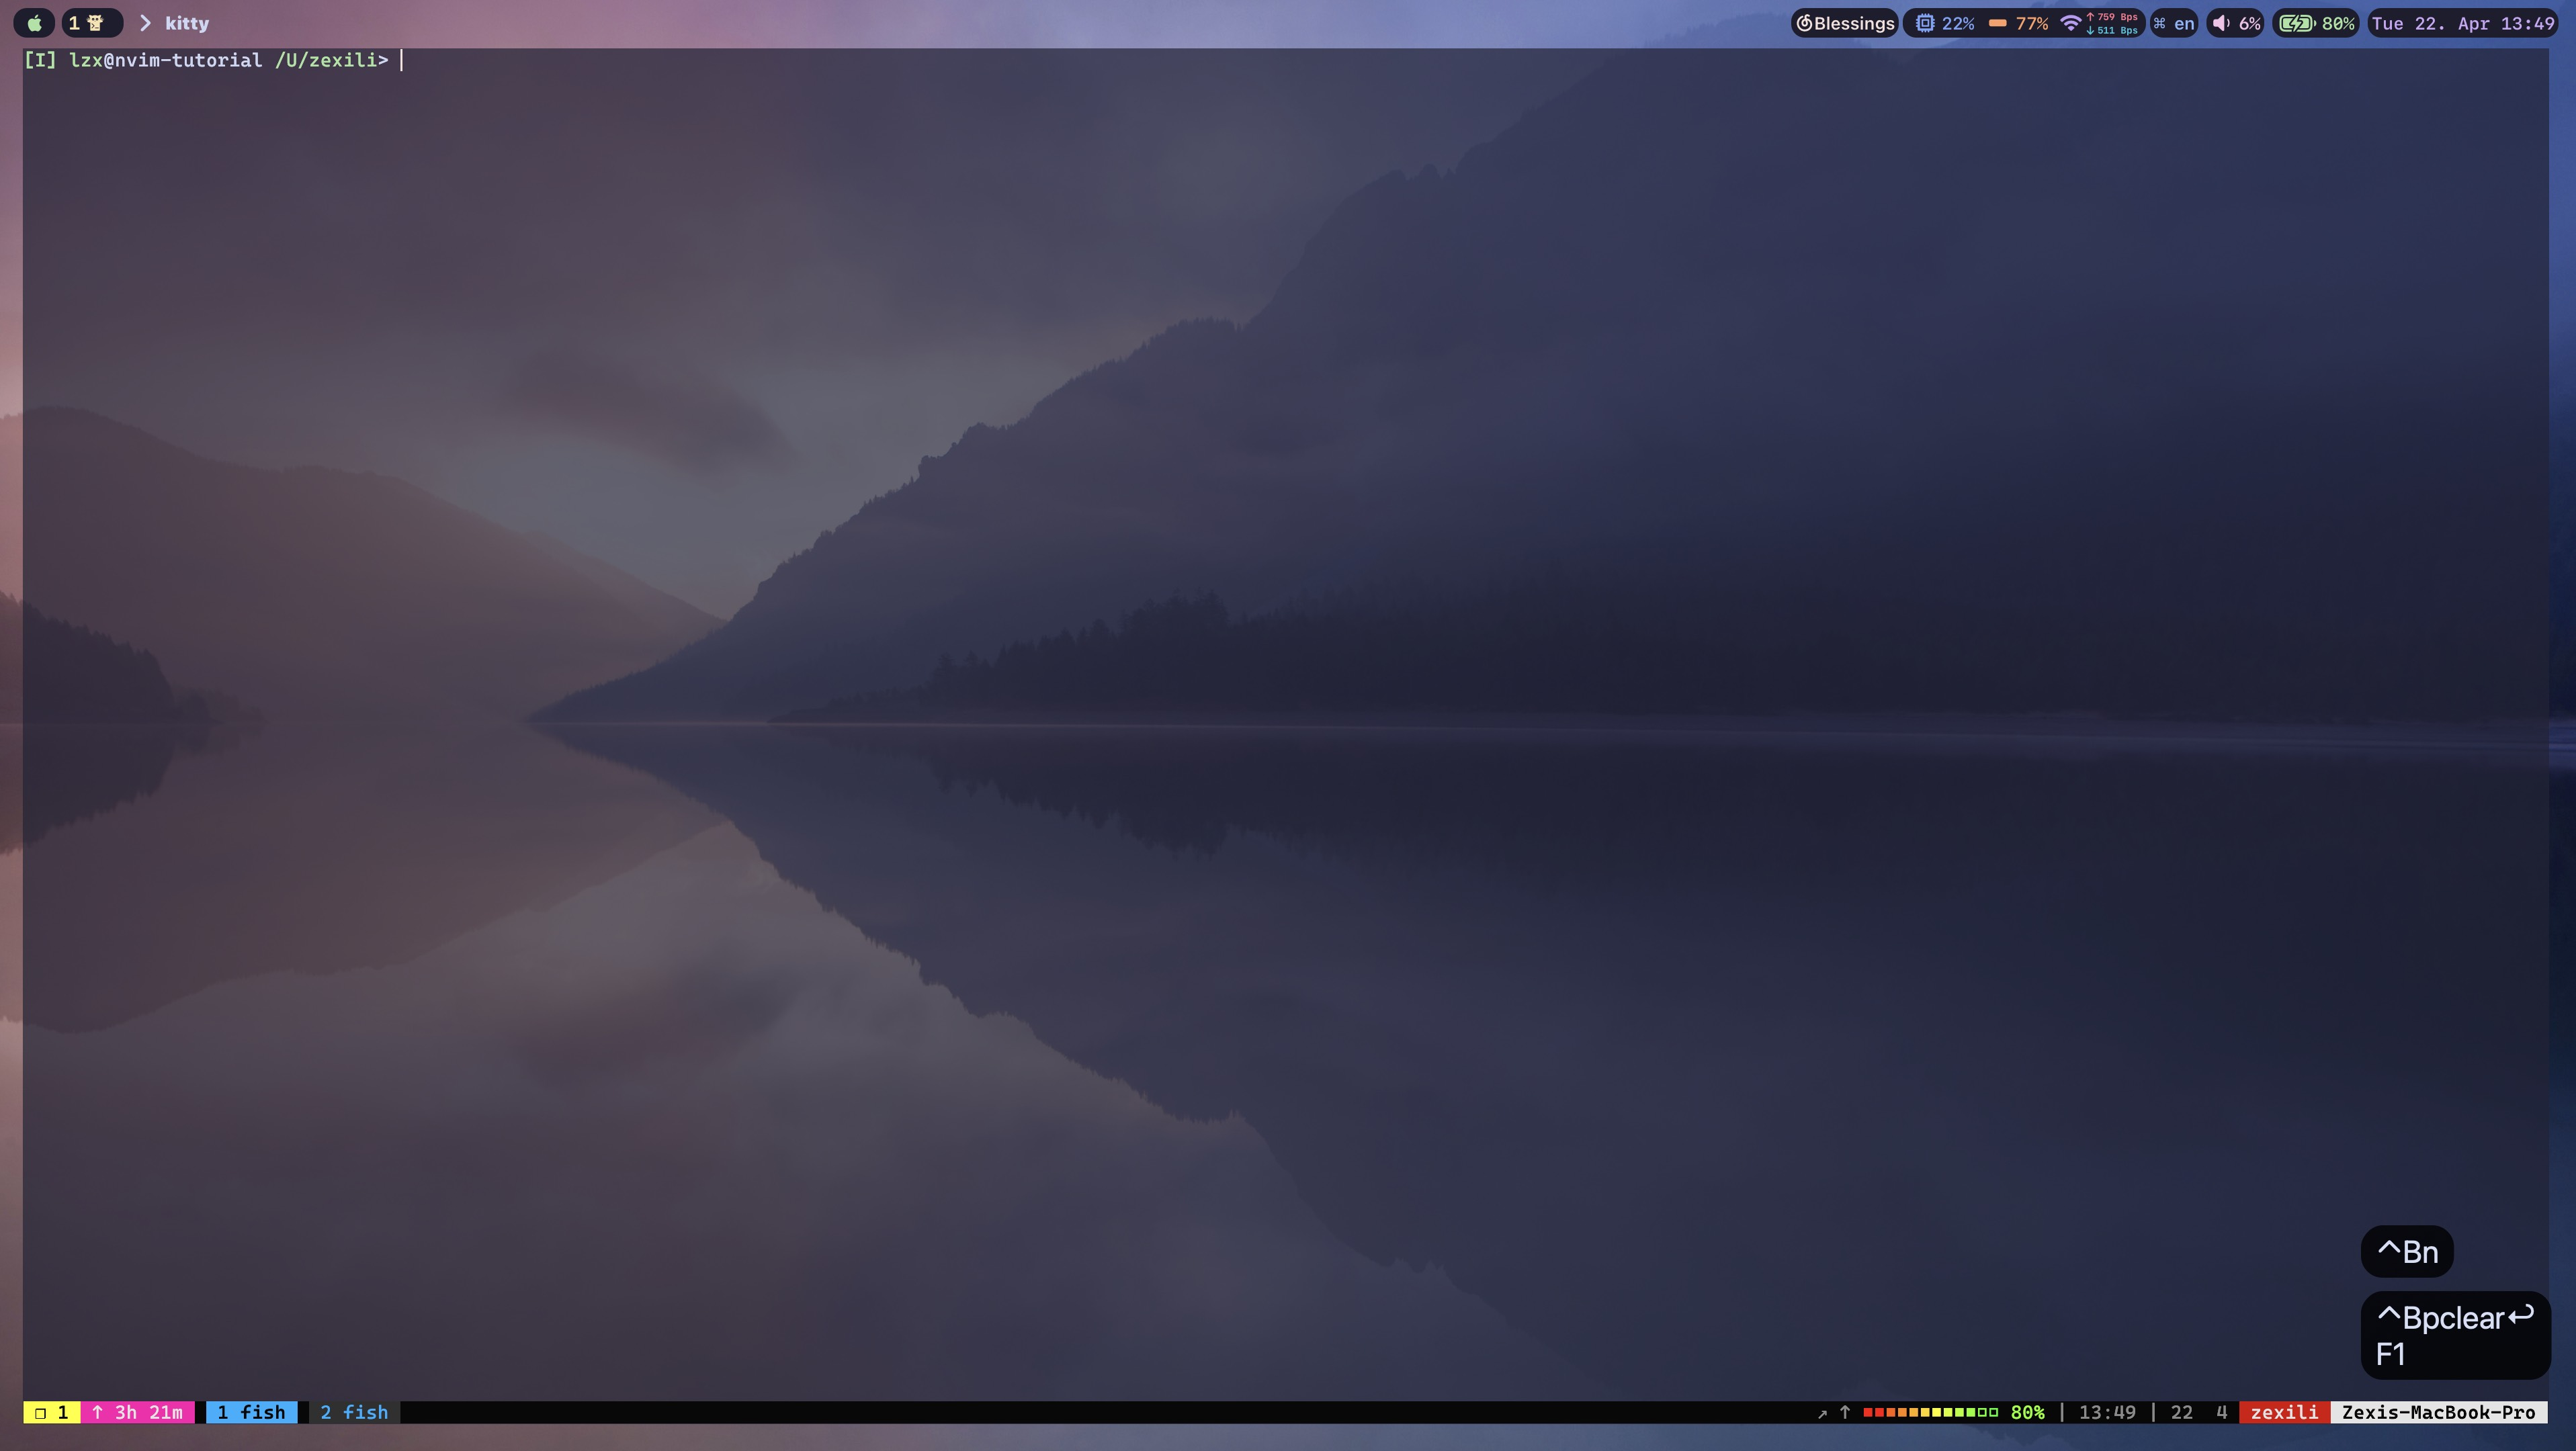
\includegraphics[width=\linewidth]{./Figures/Screenshot.jpg}
        % \caption{界面介绍}%
      \end{figure}
    \end{column}
  \end{columns}
\end{frame}

\begin{frame}{大纲}
  \tableofcontents
\end{frame}
% Current section
\AtBeginSection[ ]
{
  \begin{frame}{大纲}
    \tableofcontents[currentsection]
  \end{frame}
}

\section{Neovim介绍}
  \begin{frame}\frametitle{Neovim介绍}
    Neovim的历史
    \begin{itemize}
      \item vi (1976):名字取自Visual的前两个字母,vi发明的多编辑模式作为文本编辑的经典一直延续至今 % ChkTeX 19
      \item vim (1991):Vi IMproved,在vi的基础上新增了许多功能(多窗口、语法高亮等),更加方便了用户的使用 % ChkTeX 19
      \item neovim (2014):Vim的一个分支,起因为给vim提交的一个实现多线程的补丁被拒绝,作者(们)决定自己在原先vim的代码上进行二次开发
    \end{itemize}
    Neovim与Vim的区别
    \begin{itemize}
      \item Neovim的配置用Lua描述,Vim的配置用Vimscript描述
      \item \( \cdots \)
    \end{itemize}

    \refnote{Reference:}
    \footnotetext{[1] https://en.wikipedia.org/wiki/Vi\_(text\_editor)}
    \footnotetext{[2] https://en.wikipedia.org/wiki/Vim\_(text\_editor)}
  \end{frame}

\section{所用工具的介绍及下载}
  \subsection{Neovim}
    \begin{frame}[containsverbatim]{Neovim下载}
      准备工作:
      \begin{itemize}
        \item git
        \item \link{fish}{https://fishshell.com/}(可选):好看的shell
      \end{itemize}

      Neovim下载: \url{https://github.com/neovim/neovim/blob/master/INSTALL.md\#ubuntu}

      将下载步骤中的
      \begin{lstlisting}
    sudo add-apt-repository ppa:neovim-ppa/stable
    sudo apt-get install python-dev python-pip python3-dev python3-pip
      \end{lstlisting}
      换成
      \begin{lstlisting}
    sudo add-apt-repository ppa:neovim-ppa/unstable
    sudo apt-get install python3-dev python3-pip
      \end{lstlisting}
    \end{frame}

    \begin{frame}[containsverbatim]{配置文件结构}
      \begin{lstlisting}[language=bash]
      # ~/.config/nvim/
      .
      ├── init.lua # entrance
      └── lua
          ├── config
          │   └── lazy.lua # Lazy.nvim config
          └── plugins
              └── treesitter.lua # nvim-treesitter config (next chapter)
      \end{lstlisting}

    \end{frame}

  \subsection{Lazy.nvim}
    \begin{frame}[containsverbatim]{Lazy.nvim - 插件管理器}
      \link{Lazy.nvim}{https://github.com/folke/lazy.nvim}:一个现代的Neovim插件管理器

      由folke制作

      Requirements:
      % \begin{itemize}[label={\color{red}{\protect\ding{\value*}}}]
      \begin{itemize}
        \item Neovim >= 0.8.0 (needs to be built with LuaJIT)
        \item Git >= 2.19.0 (for partial clones support)
        \item a Nerd Font (optional)
        \item luarocks to install rockspecs. You can remove rockspec from opts.pkg.sources to disable this feature.
          \begin{lstlisting}
  sudo apt install luarocks
          \end{lstlisting}
      \end{itemize}

    \end{frame}

\section{所用工具的配置}
  \subsection{Neovim}
    \begin{frame}[fragile]{Neovim配置}
      \begin{lstlisting}[language={[5.1]lua}]
    -- ~/.config/nvim/init.lua

    vim.wo.cursorline = true
    -- Display tabs and trailing spaces
    vim.opt.list = true
    vim.opt.listchars = { tab = ">-", trail = "-" }

    -- Make sure to setup `mapleader` and `maplocalleader` before
    -- loading lazy.nvim so that mappings are correct.
    -- This is also a good place to setup other settings (vim.opt)
    vim.g.mapleader = " "
    vim.g.maplocalleader = "\\"
      \end{lstlisting}
    \end{frame}
  \subsection{Lazy.nvim}
    \begin{frame}[fragile]{Lazy.nvim配置}
      \begin{lstlisting}[language={[5.1]lua}]
    -- ~/.config/nvim/lua/config/lazy.lua

    require("lazy").setup({
      ...
      ui = {
        -- The border to use for the UI window. Accepts same border values as |nvim_open_win()|.
        border = "rounded",
      }
      ...
    }

    vim.keymap.set("n", "<leader>L", "<CMD>Lazy<CR>", { desc = "[Lazy] Open Lazy.nvim" })
      \end{lstlisting}
    \end{frame}

\section{拓展材料}
  \begin{frame}[fragile]{拓展材料}
    \begin{itemize}
      \item Neovim官方教程
        \begin{itemize}
          \item 在Neovim中输入 \lstinline[style=nvim]{:Tutor} 命令
        \end{itemize}
      \item \link{Vim Adventures}{https://vim-adventures.com/}:通过游戏的方式学习Vim
        \begin{figure}[H]
          \centering
          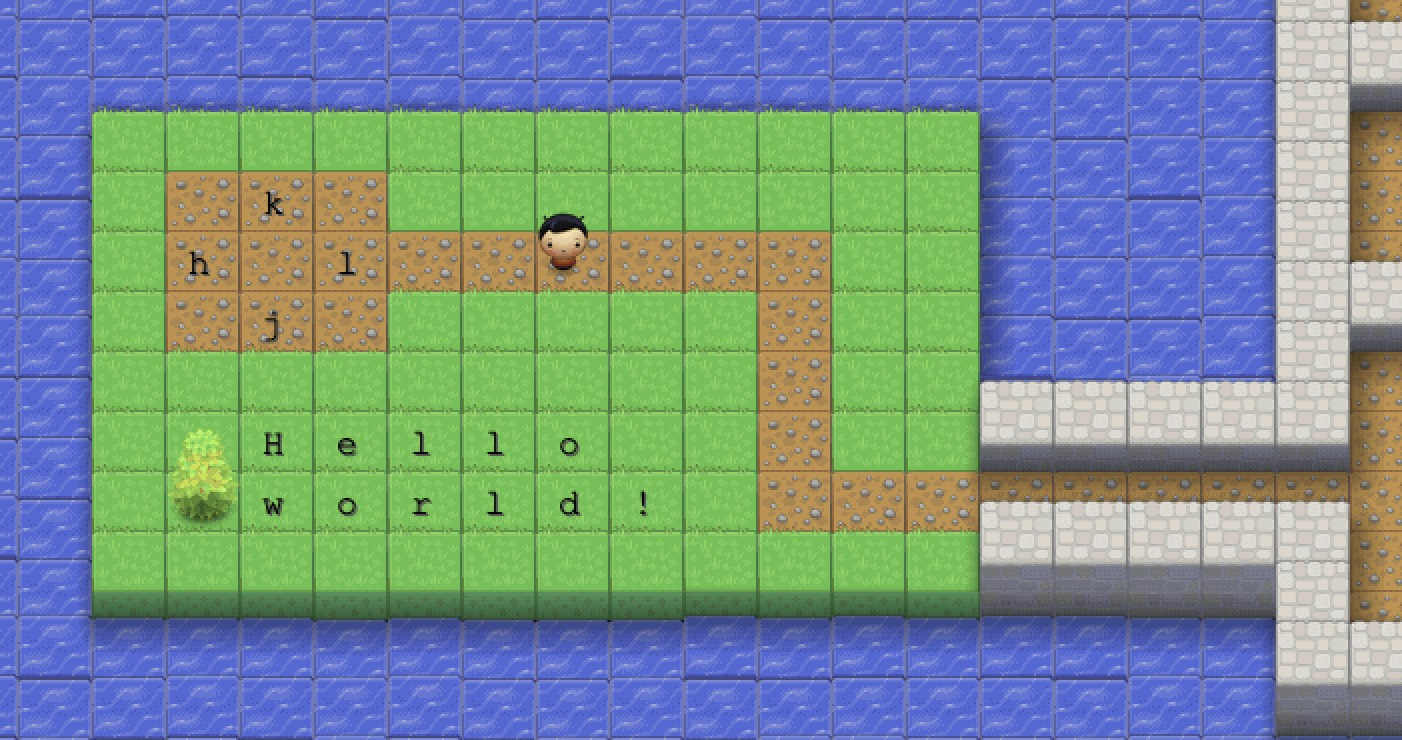
\includegraphics[width=0.4\linewidth]{./Figures/Vim_Adventure.jpg}
        \end{figure}
      \item Neovim帮助手册
        \begin{itemize}
          \item 在Neovim中输入 \lstinline[style=nvim]{:help} 命令
        \end{itemize}
    \end{itemize}
  \end{frame}

  \begin{frame}{Thanks}
    配色方案:
    \begin{itemize}
      \item \link{Catppuccin}{https://catppuccin.com/} 
\includegraphics[height=10pt]{./Figures/Catppuccin_logo.png}
      \item \link{Catppuccin for beamer}{https://github.com/atticus-sullivan/beamercolortheme}
    \end{itemize}
  \end{frame}

\end{document}
